\documentclass[11pt]{article}
\usepackage{graphicx}
\input def.tex
\begin{document}
%EDIT THIS FILE AND FILL IN THE RELEVANT DETAILS.
\input hct_title.tex

%ENTER CYCLE APPLYING FOR (No. & PERIOD); ENTER DATE OF PROPOSAL SUBMISSION
{\bf Cycle applying for: 2015-Cycle2}~~~~~~~\hfil Date: \hfil\\
%
%ENTER TITLE OF PROPOSAL AFTER CURLY BRACKETS
%
\\
{\bf 1. Title of the proposal : Late time observations of the nearby SN2014J in optical  and near infrared} 

%IN THE FOLLOWING, CHANGE "NO" to "YES" WHERE APPLICABLE.
%
\NO~Short term \hfil \NO~Long term \hfil Number of cycles/nights: ~~~~\hfil\\
\NO~Ongoing proposal \hfil Previous proposal code(s):~~~~~~~~~~~~~\hfil~~~~\\
\YES~Thesis topic \hfil Expected year of thesis submission: 2016  \hfil~~~\\
{\bf \small {If proposal is intended to support a Ph.\ D.\ project, please
include, in addition to the Scientific Justification, a brief outline of the 
Ph.\ D.\ project and the relevance of the proposal to the Ph.\ D.\ project}}\\

%
%LIST NAMES OF PROPOSERS WITH E-MAIL ADDRESS.
%
{\bf 2. List of Proposers: } {\sl indicate PI(s)}\\[1mm]
\begin{tabular}{|p{2in}|p{2in}|p{1.5in}|p{0.8in}|}
\hline
Proposer & Affiliation & e-mail & Will be present for observations?\\
\hline
S. Dhawan& ESO & sdhawan@eso.org& no\\ \hline
 B. Leibundgut & ESO &bleibund@eso.org & no\\ \hline
S. Taubenberger & ESO & tauben@mpa-garching.mpg.de & no\\ \hline
W. Kerzendorf & ESO & wkerzend@eso.org & no\\ \hline
K. Maguire & ESO & maguirek@eso.org & no\\ \hline
J. Spyromilio & ESO & jspyromi@eso.org & no\\ \hline
\end{tabular}

%NAME AND ADDRESS OF PROPOSER FOR CONTACT
%
{\bf 3. Contact Name \& Address: }\\
European Southern Observatory,
Karl Schwarzschild Strasse, 2
Garching bei M{\"u}nchen, 85748, 
Germany
\\
Telephone:\\
Fax:\\
%GIVE A BRIEF ABSTRACT OF THE PROPOSAL
%
\textbf{ 4. Abstract: }
Type Ia supernovae (SN Ia) have been used as exceptional cosmological distance indicators. They are thermonuclear explosions of white dwarfs (WDs) in a binary system. However, there are several unanswered questions regarding the physics  of SN Ia, for e.g. the progenitor mass, explosion mechanism and the nature of the companion. The late time photometry, in the optical and near infrared (NIR), is a crucial tool in answering some of these questions. At late times, the ejecta are transparent to $\gamma$ rays and the light curve is powered by positron kinetic energy. The late time (pseudo-) bolometric light curve allows us to determine the positron escape fraction. The extent of trapping depends on the strength and configuration of the magnetic field. A strong, tangled magnetic field would arise from a Chandrasekhar mass WD whereas a weak magnetic field would indicate an edge-lit detonation of a sub-Chandrasekhar WD. Thus, the late time bolometric light curve is an efficient tool in constraining the explosion scenario
Moreover, at late times, we can test the model prediction of the presence of an Infrared Catastrophe (IRC), wherein there is a sharp decline the optical and NIR flux, which offers insight into the excitation state of the ejecta. SN2014J, the closest SNIa in over 4 decades, offers us an ideal laboratory understand SNe using late time data. %Hence, we propose for multi-epoch optical and NIR photometry
 %The late phase photometry allows us to study some important aspects like the production of radioactive and stable elements and their distribution in the ejecta. In the late phases ($>$ 400 days), the SN is transparent to $\gamma$ rays and the light curve is powered by positrons. The extent of positron trapping can be constrained from the slope of the late time (pseudo-)bolometric light curve, with a steeper slope indicating a lesser extent of $e^{+}$ trapping. This allows us to distinguish between different configurations of the magnetic field in the ejecta, and hence, distinguish between predictions from different explosion models. 
%At late times, we can probe the inner layers of the ejecta. The late time light curve is sensitive to the ionisation and excitation state of the ejecta. This allows us to observe the predicted Infrared Catastrophe (IRC), wherein a sharp decrease is seen in the optical and near infrared (NIR) flux. SN2014J, the closest SNIa in over 4 decades, offers us an ideal laboratory to look for the presence of an IRC. Hence, we propose for multi-epoch optical and NIR photometry of SN2014J.
% Probing the occurrence of an Infrared Catastrophe at these epochs allows us to understand the ejecta temperature and density distribution. We also plan to submit follow-up proposals to observe SN2014J at epochs $>$ +700 days since there are no measurements of an SNIa out to such late phases in the NIR. 
\\ 
%BEGIN ABSTRACT
\\
\\
\\
\\
\\
\\
\\
\\
\\
\\
\\
%END ABSTRACT

%\newpage 
{\it HCT Proposal}\hskip 5cm {\it Page 2} \hfill {\it Cover page (contd)}\\[1mm]
\hrule

{\bf 5. Status of ongoing / previous proposals:}\\ 
%FIRST TIME APPLICANTS MAY ENTER `NA'
{\sl \small {1. Please give a brief status report of any previous HCT proposals, and
attach any preprint/reprint based on these HCT observations\\
2. If your proposal is long-term / on-going, briefly state the status of the
proposal, mentioning the progress with respect to the science goals.}}\\
{\bf \small {NOTE: Incomplete proposals are likely to be given low priority
or rejected}
}
\\
N/A
\\
\\
\\
\\
\\
\\
\\
\\
\\



\hrule
{\bf For official purpose only}

{\it Referee's comments:}\\
\\
\\
\\
\\
\\
\\
\\
\\
{\it Science feasibility:} \hfil {\it Technical feasibility:} \hfil \\

{\it Grade of the proposal:} \hfil \\

{\it Dates allotted:}

\newpage
{\it HCT Proposal}\hskip 5cm {\it Page 3} \hfill {\it Observing Details}\\[1mm]
\hrule
{\bf 6. Scheduling request: }~~~~~\\
%
%IN THE FOLLOWING LINES, CHANGE "NO" to "YES" TO INDICATE THE DESIRED 
%SCHEDULING REQUEST 

\NO~Dark night is essential \hfil \NO~Grey night is all right~~~~~\\
\NO~Bright night is all right \hfil \YES~Time-critical observations\\
\NO~Target of Opportunity \hfil \YES~Other (specify)  We request dark night for optical observations only, NIR can be conducted in grey or bright conditions~~~~~~~~~~~~~\\

\begin{tabular}[t]{p{9cm}p{9cm}}
{No. of nights requested: 6 hrs}(total exposure time and calculations in section \textbf{10})\\
{Preferred dates: May 1st to June 30th} & {Impossible dates: June 30 to August 31}\\

\end{tabular} \\ 

{\bf 7. Justification for scheduling request: }\\
SN2014J has the lowest visibility between end of June and end of September, hence, we request for the 3 observations in May and June,  with a cadence of $\sim$ 25-30 days. Hence, we have requested for time-critical observations

We request dark nights for the optical observations since they significantly reduce exposure times in the optical. With 1 mag  sky brightness above dark sky, the exposures increase by a factor of 2. We would like to observe the SN in $1^{"}$ or better seeing. 
\\

{\bf 8. Instrument:} {\sl check all that apply}\\
%
% IN THE FOLLOWING LINES, CHANGE "NO" to "YES" TO INDICATE THE REQUIRED
% INSTRUMENT(S)
\YES~HFOSC\\
\NO~Optical CCD Imager\\
\YES~TIFR Near-IR Spectrometer (TIRSPEC)\\

{\bf 9. Mode of Observation:} {\sl check all that apply}\\ 
%
% IN THE FOLLOWING LINES, CHANGE "NO" to "YES" TO SPECIFY THE MODE(S) OF
% OBSERVATION
\YES~Imaging
\NO~Spectroscopy
\\

{\bf 10. Brief description of observations: } \\
We request observations of the target at intervals of 25-30 days, with the first epoch in May. For each observation date, we would like to observe the SN in the  B to K filters with the HFOSC(BVRI) and TIRSPEC (JHK) instruments  \\

The total number of observations requested is 3 epochs.\\

To calculate the exposures in the optical, we normalise the maximum light observations of SN2001el (a well-observed normal Ia) to the peak of SN2014J in the $BVRI$ filters. As a result, we use the predicted fading of SN2001el to get the magnitudes at these late phases. 
We summarise the exposure times in  table \ref{tab:exp}
Note: we use the Liverpool Telescope's (LT) exposure time calculator (ETC) to get these estimates since there isn't an ETC for HFOSC and the LT has a similar diameter of the primary mirror. 
%\bigskip

\begin{tabular}{lllll|}
%\caption{Exposure times }
Filter & Magnitude & Exp. Time (s; dark, $1^{"}$)  & Exposure (s; dark + 1 mag, $1^{"}$) \\
\hline
B	& 21.3  & 300 & 600 \\
V	& 20.3 & 100 & 200 \\
R	&  20.6 & 150	&  300   \\
I	&   18.0  & 30 & 30 \\
\hline
\label{tab:exp}
\end{tabular}
\newpage
For the optical the total exposure time is close to 10 mins. We estimate overheads of 10 mins. 

For  calculations in the NIR we use the TIRSPEC exposure time calculator. For our desired signal to noise, we require 5 dithers of 6 frames with 15\,s exposures. Since, we require off source images for sky subtraction, we would like to split this observation into two sequences of 5 dithers with 3 frames. 
Hence, we would obtain a total exposure time of 450\,s 
We multiply this by a factor of 3 to get the overheads for the on-source and off-source sequences. Hence, the total time in each filter for the observation will be close to 25 minutes. Thus, we require 1.5 hours for each epoch.

The total time for each epoch, optical + IR is  a little less than 2 hours.

 Hence, the total time requested for the semester is 3 $\times$ 2 = 6 hours. 


We would like to mention that this proposal is part of an observing campaign to compile a detailed late time dataset of SN2014J at very late epochs, starting with observations at $\sim +$ 450 days and extending out to epochs beyond $+$700 days, for which there are almost no observations of a normal SNIa. 

For this proposal, the SN will  in the phase range between $+450$-$+580$ days during the observing cycle.  We request for 3 epochs of observation in order to strictly constrain the evolution in the optical and NIR, within this phase range. 
\\
\\
\\
\\
{\bf 11. Plans for data reduction and analysis: }
We plan to use the available reduction software for TIRSPEC and HFOSC to reduce the images .
We have downloaded the photometry templates %kidhar se aaya be 
 for M82 for accurate host galaxy subtraction. 
We currently have routines ready for the bolometric light curve calculation which have also been tested on data for other projects (Dhawan et al. in prep). 
 \\


%\newpage
{\it HCT Proposal}\hskip 5cm {\it Page 4} \hfill {\it Observing Details (contd)}\\[1mm]
\hrule
{\bf 12. Instrument Resource Requirements:}\\[1mm]
% IN THE FOLLOWING LINES, CHANGE "NO" to "YES" TO INDICATE THE REQUIREMENT(S).

{\bf HFOSC}\\
{\bfs Broad Band Filters:} \NO~U \YES~B \YES~V \YES~R \YES~I \NO~I$_c$ 
\NO~$z$\\ [1mm]
%{\bfs Narrow Band Filters:} \NO~486.1(10) \NO~500.7(10) \NO~656.3(10) 
%\NO~672.4(10) \NO~656.3(50) \\[1mm]
%{\bfs Grisms:} \NO~Gr.5 \NO~Gr.7 \NO~Gr.8 \NO~Gr.9 \NO~Gr.10 \NO~Gr.11
%\NO~Gr.12 \NO~Gr.14 \NO~Gr.15 \NO~Gr.17\\[1mm]
%{\bfs Slits:} \NO~67(s) \NO~67(l) \NO~100(m) \NO~100(l) \NO~134(s) 
%\NO~134(l) \NO~167(l) \NO~335(l) \NO~1340(l)\\[1mm]
\iffalse
{\bf Optical CCD Imager}\\ 
{\bfs Broad Band Filters:} \NO~U \NO~B \NO~V \NO~R \NO~I \NO~I$_c$ 
\NO~$z$\\[1mm]
{\bfs Narrow Band Filters:} \NO~372.7(5) \NO~486.1(5) \NO~500.7(5) 
\NO~656.3(5) \NO~664.3(10) \NO~672.4(10) \NO~680.4(10) \NO~688.4(10) 
\NO~696.4(10) \NO~704.4(10) \NO~712.4(10)\\[1mm]
\fi
{\bf TIRSPEC}\\
{\bfs Broad Band Filters:} \YES~J \YES~H \YES~K$_{\rm s}$ \\ [1mm]
%{\bfs Narrow Band Filters:} \NO~Methane off (1.584, 3.6\%) \NO~[Fe II] (1.645, 1.6\%) \NO~Methane on (1.654, 4.0\%)
%\NO~H2(1-0) (2.1239, 2.0\%) \NO~Br$\gamma$ (2.166, 0.98\%) \NO~K-cont (2.273, 1.73\%) \NO~CO(2-0) (2.287, 1.33\%) \\[1mm]
%{\bfs Single Order Dispersers:} \NO~Y (1.02--1.20) \NO~J (1.21--1.48) \NO~H (1.49--1.78) \NO~K (2.04--2.35)\\[1mm]
%{\bfs Cross Dispersers:} \NO~YJ (1.02--1.49) \NO~HK (1.50--2.45)\\[1mm]
%{\bfs Slits:} \NO~1"(s) \NO~1"(l), \NO~1.5"(s) \NO~1.5"(l) \NO~2"(s)
%\NO~2"(l) \NO~3"(s) \NO~3"(l) \NO~8"(s) \NO~8"(l)\\[1mm]

% LIST THE OBJECTS PROPOSED TO BE OBSERVED BELOW. PLEASE NOTE THAT THE PROPOSAL
% MAY BE REJECTED IF NO LIST IS PROVIDED.
%

{\bf 13. List of objects: (essential)}\\

\begin{tabular}{|p{1in}|p{1.5in}|p{1.5in}|p{0.5in}|p{0.5in}|p{0.5in}|}
\hline
Name & RA (hh mm ss)& Dec (dd mm ss) & Epoch & $V$ mag & size$^*$ \\
\hline
SN2014J & 09 55 42.12 & +69 40 25.9  &  J2000 & 20.3 &  N/A  \\\hline
\hline
 \multicolumn{6}{l}{*for extended objects}\\
\end{tabular}

\newpage
{\it HCT Proposal}\hskip 5cm {\it Page 5} \hfill {\it Scientific Justification}\\[1mm]
\hrule
{\bf 14. Scientific Justification:} {\sl Type Ia supernovae (SN Ia) are thermonuclear explosions of white dwarfs in a binary system.  It is known that their light curves are powered by the decay of $^{56}$Ni at early times and its daughter nuclide $^{56}Co$ at late epochs (Colgate $\&$ Mckee [1969]; Arnett [1982]).  There are, however, several unanswered questions regarding the physics of SN Ia. For e.g., the nature of the binary companion is unknown, with two leading possibilities of a main sequence/red giant (single-degenerate) or another white dwarf (WD; double degenerate) companion. Recent studies have also shown that SN Ia do not all explode at the Chandrasekhar mass, as was originally thought, and a significant fraction of them are sub-Chandrasekhar explosions (Stritzinger et al. [2006], Scalzo et al. [2014]) which challenges the notion of all SN Ia being Chandrasekhar mass explosions and indicates a possible diversity in the progenitor channel.    %The late time photometry is instrumental in distinguishing different progenitor scenarios based on the predictions of their late time behaviour. 

%Their use as distance indicators in cosmology has led to dedicated efforts to obtain data for large samples of SNeIa. Most of the assimilated data for the SNe~Ia are directed towards understanding them during the early photospheric phase. At late phases, the $\gamma$ ray escape fraction increases and most of the light curve is powered by the positrons. Hence, these late-phases of these SNe offer other opportunities to study the physics of these explosions, for eg. constraining the geometry of the magnetic field.
\textbf{Progenitor scenarios and the magnetic field:}

At late times, the ejecta is transparent to the $\gamma$ rays and most of the light curve is powered by positrons. The extent of positron trapping in the ejecta is determined by the strength and configuration of the magnetic field in the ejecta, with a stronger, tangled field yielding a higher extent of positron trapping. Detonation models of sub-Chandrasekhar WDs predict a weak, radially combed magnetic field, whereas Chandrasekhar mass explosions, due to high turbulence, predict a  stronger, tangled magnetic field (Ruiz-Lapuente $\&$ Spruit 1998). Hence, we can use the positron escape fraction to constrain the explosion scenario for SN2014J. The late time (pseudo-)bolometric light curve is sensitive to the extent of positron trapping, with a flatter slope indicating more positrons are trapped. If indeed, most of the positrons are trapped in the ejecta, the late time bolometric light curve can also be used to estimate the amount of $^{56}Ni$ ejected in the SN. These observations, in principle, can also be used to constrain the contribution these positrons make to the galactic 511 keV line (Milne et al. [1999]).  In figure \ref{fig:bol}, we show the (pseudo-)bolometric light curve for SN2001el from Stritzinger $\&$ Sollerman [2007], compared to their toy model. Their bolometric light curve only extends out to $\sim$  +440 days. We propose to extend these observations to +500 days (in this semester) and even later phases (over the long term of 3 semesters). 
%The fraction of positron energy deposited into the ejecta depends on the magnetic field configuration. A high positron trapping fraction strongly disfavours a weak or radially combed magnetic field. Thus, the late-time (pseudo-)bolometric light curve (integrated from filters B to K) is an efficient tool in constraining the configuration of the magnetic field in the SNe and, in principle can constrain the contribution these positrons make to the galactic 511 keV line. 

\textbf{Infrared Catastrophe:}

The exponential decline in the heating due to radioactive decay and the flattening of the cooling curve at late times lead to the ejecta temperature dropping below a threshold value and hence, to a dramatic shift in the excitation state, such that only the ground state levels are populated. This leads to a significant decrease in the flux in the optical and NIR filters, with most of the emission shifted to the mid-IR region and is known as the the Infrared Catastrophe (IRC; Axelrod 1980). Theoretical models   predict an IRC to occur at $\sim$ +500 days. Observations of SN2001el do not extend to late enough phases to draw conclusions about the presence of an IRC. Very late time observations of SN2011fe in the optical by Kerzendorf et al.[2014] ($\sim$ +900\,d) show that there in no evidence for an IRC in their data (see figure \ref{fig:11fe}). However, there are only 2 observations at +550\,d and +930\,d, hence, they cannot rule out the possibility of an IRC occurring in the intermediate phase ranges between their two observations or at epochs earlier than +550 \,d. We propose to monitor SN2014J starting from $\sim$ +450\,d and see whether the IRC occurs in the ejecta. The absence of an IRC would mean that at least part of the ejecta is above the threshold temperature and would indicate that the ejecta could have a clumpy distribution.
 %However, due to sparse sampling at these epochs, one cannot exclude the possibility of an IRC having occurred during the epochs where the SN wasn't observed. For SN2003hv (Leloudas et al. [2009]), a possibility of an IRC having occurred in the innermost layers of the ejecta is proposed to explain the late time data. In figure \ref{fig:11fe}, we show the comparison of the theoretical models with the pseudo-bolometric light curve of SN2011fe. There is no signature of an IRC. Hence, a good sampling at such late times is crucial to discerning the presence of an IRC, and removing the tension between the models and observations. This will, therefore, shed light on the physical conditions in the ejecta. 
 
%\textbf{Late light curve morphology}:

%A few recent studies have shown that SN Ia show a flattening of the NIR light curve at a few hundred days past maximum light . This indicates a significant contribution of the NIR to the bolometric flux at late times.  For most of these objects, in the phase range from +400  to +700 days, the light curves have very sparse sampling. By observing SN2014J with a cadence of $\sim$ 30 days, we would like to present firm constraints on the evolution of the light curve at the late epochs. This is also important to constrain the presence of an IRC and distinguish between different theoretical models based on their prediction of the late time light curve.  %why? or rather, how?

%However, there objects with such late time data have very sparse sampling and no coverage beyond $\sim$ +700 days. 

There are very few  SN Ia with late time data, especially in the NIR. SN2014J, the nearest supernova in over 4 decades provides a unique laboratory to study a normal SN Ia out to late phases. Near-maximum observations of the SN have led to epochal discoveries, for e.g. the first observation of the $^{56}Co$ line in the $\gamma$ rays. There exist excellent early time datasets for the SN with publicly available multi-band light curves, spectral time series in the optical and NIR which complement the late time observations we are proposing for. The multi-band photometry and polarimetry allow us to determine accurately the absorption from host galaxy dust. 

%There are several large datasets of SNIa near maximum light. However, only a handful of objects have been observed in the late-time, nebular phase. Moreover, there is very sparse sampling of the light curve in the phase range between +400 and +700 days and there are almost no NIR observations at $\geq$ +700 days.  The proximity of SN2014J means its bright, even at late epochs. Thus, a time-sampling of $\sim$ 30-50 days along with observations at epochs $\geq$ +700 days will allow us to understand the behaviour of a normal SNIa out to very late epochs. This would be the first such dataset for an SNIa. 

%We would like to note that the proposed optical and NIR observations provide a stand alone dataset to achieve our science goals  %motherhood?? 
\newpage

%We would like to note that these proposed observations will be taken in conjunction with multi-epoch optical spectroscopy from the Gran Telescopio Canarias (GTC). 

%\iffalse
\begin{thebibliography}{99}
\bibitem{Arnett1982} Arnett 
W.~D., 1982, ApJ, 253, 785

\bibitem{Axelrod80}  Axelrod T.~S., 1980, PhDT 

\bibitem{Colgate1969} Colgate S.~A., McKee C., 1969, ApJ, 157, 623 

\bibitem{K14} Kerzendorf W.~E., Taubenberger S., 
Seitenzahl I.~R., Ruiter A.~J., 2014, ApJ, 796, LL26


\bibitem{2009A&A...505..265L} Leloudas G., et al., 2009, A\&A, 505, 265 

\bibitem{1999ApJS..124..503M} Milne P.~A., The L.-S., Leising M.~D., 1999, ApJS, 124, 503 

\bibitem{1998ApJ...500..360R} Ruiz-Lapuente P., Spruit H.~C., 1998, ApJ, 500, 360 

\bibitem{Scalzo2014} 
Scalzo R., et al., 2014, MNRAS, 560 

\bibitem{2007A&A...470L...1S} Stritzinger M., Sollerman J., 2007, A\&A, 470, L1

\bibitem{Stritzinger2006} Stritzinger M., Leibundgut B., Walch S.,
Contardo G., 2006, A\&A, 450, 241 

\bibitem{T15} Taubenberger S., et al., 2015, MNRAS, 448, 
L48 

\end{thebibliography}
%\fi


\newpage
{\bf 14a. PhD project Outline:}
This proposal is intended to support part of a PhD project. The focus of the project is to understand the Near Infrared behaviour of Type Ia supernovae, with an emphasis on late time behaviour. 
The near infrared offers complementary information to the optical for understanding the physical processes in Type Ia SNe. They appear to be more uniform at longer wavelength with a scatter $< $ 0.2 mag. We have simulated light curves a high redshift for future space-based missions to forecast the constraints on cosmological parameters. 

Another, very interesting feature in the NIR light curves is the appearance of a second maximum, around 2 weeks after maximum light in $B$-band. We investigated the relation between the second maximum (specifically the timing, termed as $t_2$). We found correlations between $t_2$ and the optical decline rate ($\Delta m_{15}$). We also found that the $t_2$ is related very strongly to the post-maximum colour evolution in the optical. These correlations point to a common origin of this diversity from the large range of $^{56}Ni$ produced in the SNe. Hence, the NIR light curve at $\sim$ 2 - 3 weeks post maximum is a probe of the total radioactive nickel synthesised in the ejecta. 

In the transitional phase (a few months after maximum light), the SN is getting progressively more transparent to the $\gamma$ rays and the light curve has an increasing contribution from positrons. Along with our conducted study of the second maximum, we would like to learn about the SN from observations in the nebular phase. At these phases, we can probe the inner regions of the ejecta. While line profile measurements from spectroscopy can shed light on the ejecta distribution, the photometric measurements at $>$ +400 days are key in uncovering global parameters of the ejecta. 

%Observations of a handful of SNe in the JHK bands show a flattening of the decline in the NIR. However, since these SNe are significantly farther and fainter  than SN2014J (for e.g. SN2001el is $\sim $3 magnitudes fainter than SN2014J) there is sparse sampling at late times. Thus,  for part of the PhD, we would like to analyse data out to 
 } 
\newpage

\begin{figure}
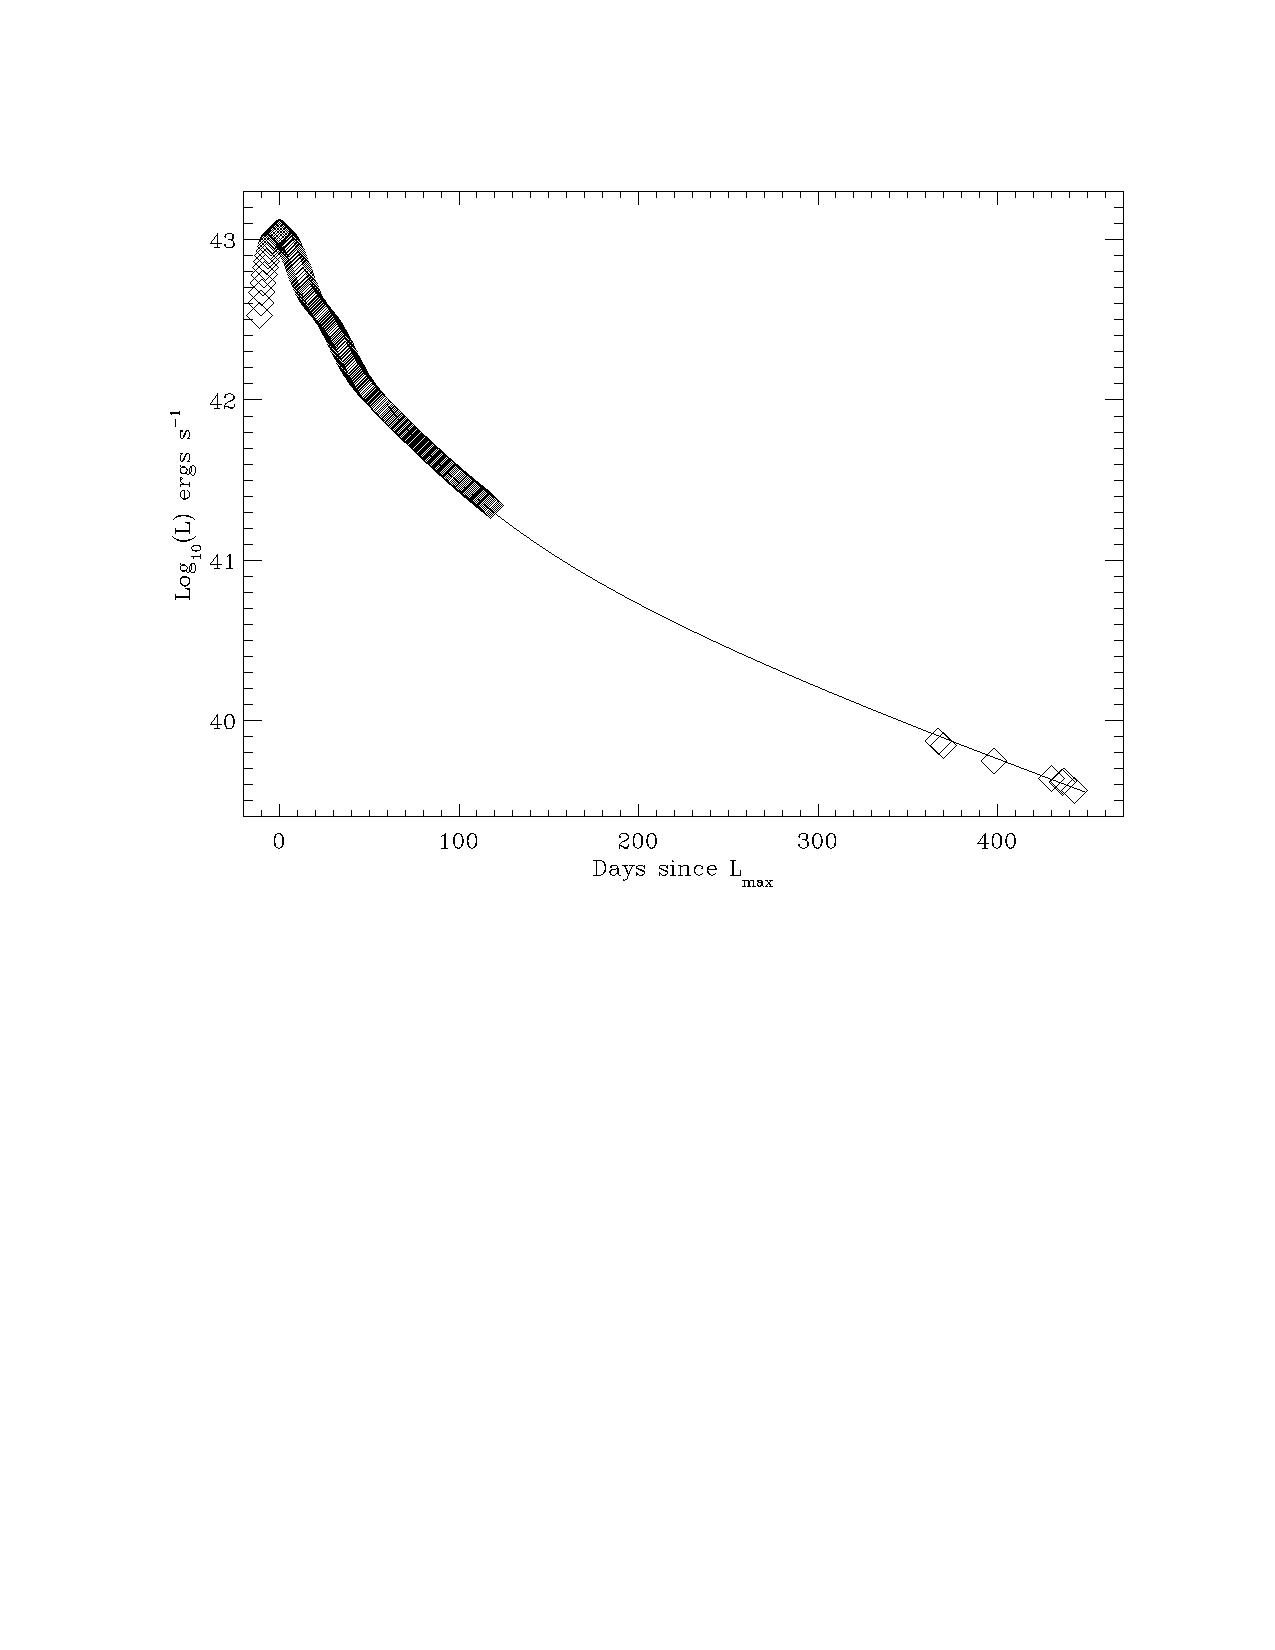
\includegraphics[width=.8\textwidth, trim=0 300 60 0]{sn01el_bol.pdf}
\caption{(Pseudo-) bolometric light curve of SN2001el from Stritzinger $\&$ Sollerman [2007]. There are very few SNe with data at later phases. The solid line is the toy model with complete positron trapping. The observed light curve follows the expectation from $^{56}$Co decay with increasing $\gamma$ ray losses. }
\label{fig:bol}
\end{figure}

\begin{figure}
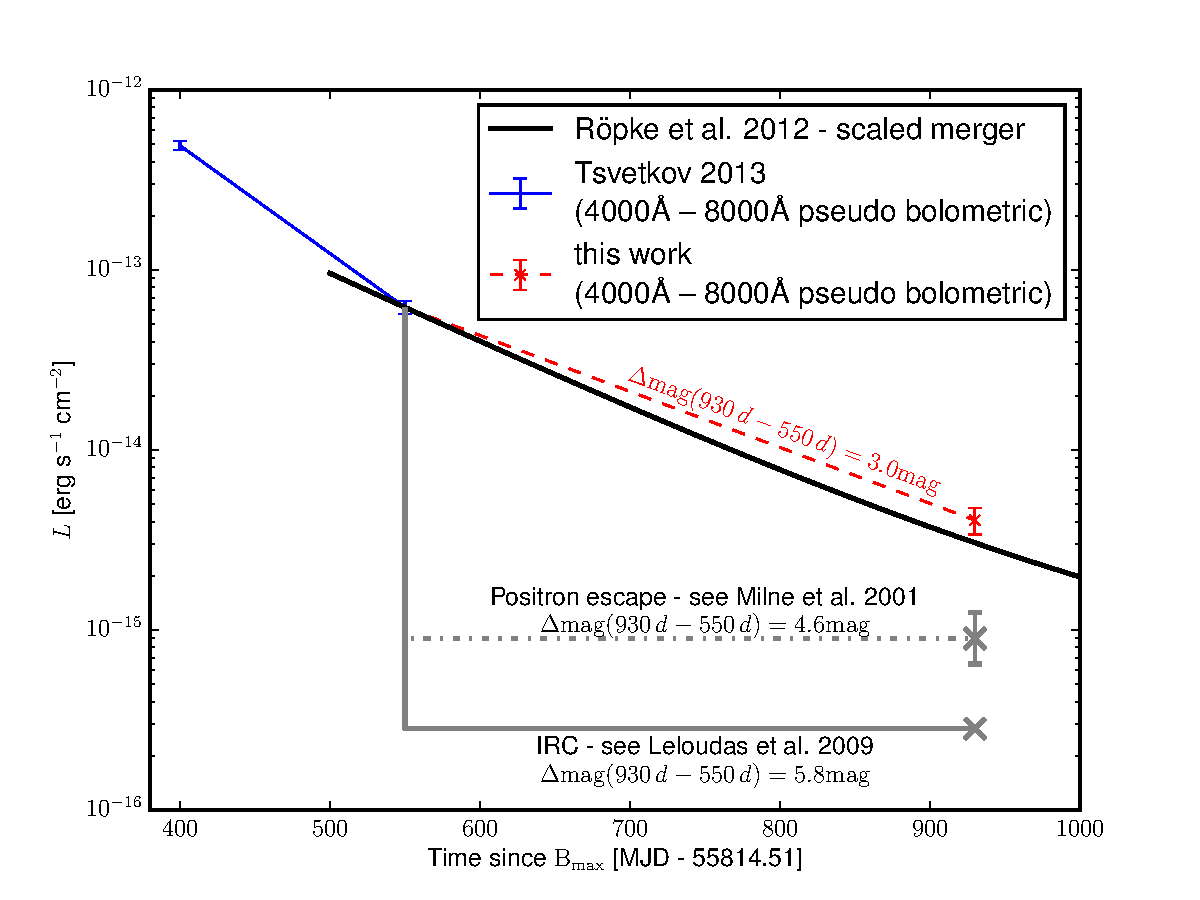
\includegraphics[width=\textwidth, trim=0 0 30 0]{sn11fe_bolom.pdf}
\caption{The (pseudo-) late time light curve of SN2011fe, the closest SN Ia before SN2014J with an excellent dataset (Kerzendorf et al. [2014]). Although models predict an Infrared Catastrophe (shift in flux from optical and NIR to mid-IR) after $\sim$ +500\,d, there is no evidence in the observations for the presence of such a shift. We note that this is only an optical pseudo-bolometric light curve ($griz$ filters). We propose to obtain optical and NIR observations for SN2014J, to better estimate the true bolometric flux.}%Light curve of SN2001el in u - K filters (Stritzinger $\&$ Sollerman 2007). The flattening of the light curve can be seen in the JHK filters.}
\label{fig:11fe}
\end{figure}
\end{document}
